\cotefile{70}

\scanpage{97}
% archive sheet number: 96
% Two long oblique cancellation strokes cross the entire written block.
% source lines 01-02, heading
\deleted{Fonctions \unsure{s.-quadriques|s.-quadratiques|bi-quadriques} nulles sur les sommets de l'icosaèdre:}

% source lines 03-06
\[
\begin{aligned}
\deleted{f(s_0)=0}&\quad\deleted{\Longrightarrow}\quad\deleted{d=0}\\
\deleted{f(s_1)=0}&\quad\deleted{\Longrightarrow}\quad\deleted{a+\lambda=0}\qquad\deleted{\text{i.e.}\quad\lambda=-a}\\
\deleted{f(s_2)=0}&\quad\deleted{\Longrightarrow}\quad\deleted{b+\mu=0}\qquad\deleted{\mu=-b}\\
\deleted{f(s_3)=0}&\quad\deleted{\Longrightarrow}\quad\deleted{c+\nu=0}\qquad\deleted{\nu=-c}
\end{aligned}
\]
% source line 07
\[
\deleted{f(x,y,z)=a(x^2-x)+b(y^2-y)+c(z^2-z)+uyz+vzx+wxy}
\]
% source line 08
\[
\deleted{f({\unsure{s|\ell}}''_3)=b(1+\alpha)\alpha+u(1+\alpha)=0}
\qquad\deleted{\underline{u=-\alpha b}}
\]
% source line 09
\[
\deleted{f(\unsure{\underline a|\widehat a|\widehat\sigma}s_1)=\deleted{\unsure{b}}(\alpha+1)(\alpha+2)(b+c)\unsure{-|+}b(\alpha+2)=0}
\]
% source lines 10-11
\[
\begin{aligned}
\deleted{\text{\unsure{d'o.|d'où.}}\quad(\alpha+1)(b+c)-b=0}
&\qquad\deleted{\text{i.e.}\quad\alpha b+(\alpha+1)c=0}\\
\deleted{\text{i.e.}\quad b=-\left(1+\frac1\alpha\right)c=-(2+\alpha)c}&
\end{aligned}
\]


\scanpage{98}
% archive sheet number: 97
% source lines 01-02; multiplication arcs above and below the factors
\figure{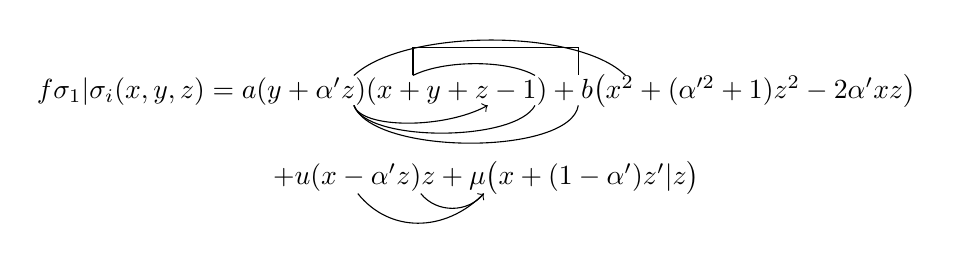
\begin{tikzpicture}[x=1cm,y=1cm]
\node[anchor=west] at (0,0) {$f\unsure{\sigma_1|\sigma_i}(x,y,z)=a(y+\alpha'z)(x+y+z-1)+b\bigl(x^2+(\alpha^{\prime 2}+1)z^2-2\alpha'xz\bigr)$};
\node[anchor=west] at (3,-1.1) {$+u(x-\alpha'z)z+\mu\bigl(x+(1-\alpha')\unsure{z'|z}\bigr)$};
\draw (4.15,.2) .. controls (4.8,.8) and (7.0,.8) .. (7.6,.2);
\draw (4.9,.2) -- (4.9,.55) -- (7.0,.55) -- (7.0,.2);
\draw (4.9,.2) .. controls (5.3,.4) and (6.1,.4) .. (6.45,.2);
\draw[->] (4.15,-.18) .. controls (4.25,-.48) and (5.3,-.48) .. (5.85,-.18);
\draw (4.15,-.18) .. controls (4.3,-.65) and (6.2,-.65) .. (6.45,-.18);
\draw (4.15,-.18) .. controls (4.4,-.82) and (6.9,-.82) .. (7.0,-.18);
\draw[->] (4.2,-1.3) .. controls (4.6,-1.8) and (5.3,-1.8) .. (5.8,-1.3);
\draw (5.0,-1.3) .. controls (5.2,-1.55) and (5.6,-1.55) .. (5.8,-1.3);
\end{tikzpicture}}
% source lines 03-05
\[
\begin{aligned}
={}&bx^2+ay^2+\bigl(a\alpha'+b(1+\alpha^{\prime 2})\inserted{\unsure{+|-}u\alpha'}\bigr)z^2\\
&+(-a\alpha)yz+(a\alpha'-2b\alpha'+u)zx+\deleted{\unsure{2}}axy\\
&+\mu x+(-a)y+\bigl(-a\alpha'+\mu(1-\alpha')\bigr)z
\end{aligned}
\]
% source line 06
\[
\deleted{\unsure{a=}}\boxed{b=a}
\]
% source lines 07-08
\[
\begin{aligned}
&a\alpha'+b(1+\alpha^{\prime 2})\unsure{-|+}u\alpha'=b\\
\text{i.e.}\quad&a\bigl(\underbrace{\alpha^{\prime 2}+\alpha'+1\deleted{\unsure{+\alpha-1|-1}}}_{\unsure{1.|10|1|0}}\bigr)=u\alpha'
\qquad\text{i.e.}\quad\boxed{u=-\alpha a}
\end{aligned}
\]
% source lines 09-14
\[
\begin{aligned}
-a\alpha&=u\qquad\text{ok}\\
a\alpha'-2b\alpha'+u&=a\quad\text{i.e.}\quad
\unsure{a}(\unsure{a\alpha'|\alpha'|4\alpha'}-2\alpha'+\underbrace{\deleted{\unsure{\alpha'}}\inserted{-\alpha}-1}_{\alpha'})=0\quad\text{ok}\\
a&=a\qquad\text{ok}\\
\boxed{\mu=-a}&\\
-a&=\mu\quad\text{ok}\\
-a\alpha'+\mu(\deleted{1}-\alpha')&=\deleted{\mu}\quad\text{i.e.}\quad
\deleted{\unsure{+a(-\alpha'-a\alpha')}}\inserted{-\alpha'(a+\mu)=0}\quad\text{ok}
\end{aligned}
\]
% source line 15
\[
f(x,y,z)=a\unsure{q|\rho}(x,y,z)
\]
% source lines 16-17
\[
\boxed{\begin{aligned}
q(x,y,z)&=x(x+y+z-1)+(y^2+z^2)\unsure{-|+}\alpha yz-(y+z)\\
&=x^2+y^2+z^2-\alpha yz+zx+xy-(x+y+z)
\end{aligned}}\tag*{(19)}
\]
% source lines 18-21
Les fonctions quadr. \unsure{invariantes} sont donc celles de la forme $aq(x,y,z)+d$, celles qui sont nulles sur $S$ sont celles de la forme $aq(x,y,z)$.


\scanpage{99}
% archive sheet number: 98
% One long oblique cancellation crosses the written calculation and conclusion.
% source lines 01-03
\[
\begin{aligned}
&\deleted{=bx^2+ay^2+\bigl[a(\alpha+2)+b(\alpha+3)+u(1+\alpha)\bigr]z^2-}\\
&\deleted{+\bigl(-2a(1+\alpha)\bigr)yz+\bigl[2b(1+\alpha)+u\bigr]zx+}\\
&\deleted{+\mu x+(-a)y+\bigl[a(1+\alpha)+\mu(2+\alpha)\bigr]z}
\end{aligned}
\]
% source line 04
\deleted{les conditions deviennent}

% source lines 05-11; left-hand system and right-hand equivalent conditions
\[
\left\{\begin{aligned}
&\deleted{a=b}\\
&\deleted{a(2\alpha+5)+u(1+\alpha)=\underset{\substack{\text{''}\\a}}{b}\quad\text{i.e.}}\\
&\deleted{-2a(1+\alpha)=u\quad\text{déjà vu}}\\
&\deleted{2b(1+\alpha)+u=0\quad\text{déjà vu}\quad(b=\unsure{0|a})}\\
&\deleted{\mu=-a}\\
&\deleted{-a=\mu\quad\text{déjà vu}}\\
&\deleted{a(1+\alpha)+\mu(2+\unsure{2|\alpha})=\mu}
\end{aligned}\right.
\qquad
\begin{gathered}
\deleted{\text{i.e.}}\quad
\left[\begin{aligned}
&\deleted{b=a}\\
&\deleted{u=2a\frac{\alpha+2}{1+\alpha}=-2a\alpha(\alpha+2)}\\
&\deleted{\hphantom{u}=-2a(\alpha+1)}
\end{aligned}\right.\\[1em]
\deleted{\text{i.e.}}\quad\left[\deleted{\mu=-a}\right.
\end{gathered}
\]
% source line 12
\[
\deleted{\text{i.e.}\quad(\mu+a)(1+\alpha)=0}
\]
% source line 13
\[
\deleted{f(x,y,z)=aq(x,y,z)\qquad\text{\unsure{où}}}
\]
% source line 14
\[
\boxed{\deleted{q(x,y,z)=x^2+y^2+z^2\deleted{\unsure{+|-}}-2(1+\alpha)yz-(x+y+z)}}
\]
% source lines 15-19
\deleted{Ainsi $q$ et la c\textsuperscript{te} $+1$ \unsure{forme|forment} une base des fonctions sous-quadratiques invariantes. Parmi celles-ci, les multiples de $q$ sont celles qui s'annulent sur les sommets de l'icosaèdre.}


\scanpage{100}
% archive sheet number: 99
% printed form: blank music staves; no printed verbal text
% source line 01, heading
Quadriques \unsure{circonscrites}

% source line 02
\[
f(x,y,z)=ax^2+by^2+cz^2+uyz+\unsure{v|\nu}zx+wxy+\lambda x+\mu y+\nu z+d
\]
% source lines 03-06
\[
\begin{aligned}
f(\unsure{s|\ell}_0)=0&\qquad\boxed{d=0}\\
f(s_1)=0&\qquad a+\lambda=0\qquad\boxed{\lambda=-a}\\
f(s_2)=0&\qquad b+\mu=0\qquad\boxed{\mu=-b}\\
f(s_3)=0&\qquad c+\nu=0\qquad\boxed{\nu=-c}
\end{aligned}
\]
% source right of lines 03-06; arrow from the four conditions
\margin{$\Rightarrow\ \begin{aligned}f(x,y,z)={}&\\a(x^2-x)&+b(y^2-y)+c(z^2-\unsure{z)}\\&+uyz+vzx+wxy\end{aligned}$}
% source lines 07-08
\[
\begin{aligned}
f(s''_3)=0&\qquad b(\alpha^{\prime 2}+\alpha')\deleted{\unsure{+u}}\unsure{-|+}u\alpha'=0
\qquad\boxed{u=\deleted{\unsure{(\alpha'+1)b}}=\boxed{-\alpha b}}\\
&u=(\alpha'+1)b=-\alpha b
\end{aligned}
\]
% source line 09, abandoned beginnings and formula above the following line
\[
f(\qquad\deleted{f=}\quad
a(x^2-x)+b(y^2-\deleted{\unsure{\alpha}}\unsure{y}-\alpha yz)+c(z^2-\unsure{z)}
\]
% source line 10
\[
f(x,y,z)=a(x^2-x)+by(y-\alpha z-1)+c(z^2-z)
+\deleted{\unsure{uyz+vzx+wxy}}\inserted{x(vz+wy)}
\]
% source lines 11-12
\[
\begin{aligned}
f(\unsure{\underline a|\widehat a|a}s'_3)=0&\qquad
b\bigl(\overbrace{1-\underbrace{\alpha(-\alpha')}_{1}-1}^{-1}\bigr)
+c\bigl(\overbrace{\alpha^{\prime 2}+\alpha'}^{1}\bigr)=0\\
&\boxed{b=c}
\end{aligned}
\]
% source lines 13-14
\[
\begin{aligned}
f(x,y,z)={}&a(x^2-x)+b\bigl(\deleted{y(y-\alpha z-1)+z(z-1)}\inserted{y^2+z^2-\alpha yz\unsure{+|-}(y+z)}\bigr)\\
&+x(vz+wy)
\end{aligned}
\]
% source lines 15-17
\[
\begin{aligned}
f(s'_3)=0&\qquad a(\alpha^{\prime 2}-\alpha')+b\bigl(-\alpha'(\underbrace{-\alpha'-\alpha-1}_{0})+0\bigr)\\
&\qquad\deleted{+\alpha'(}v\alpha'-\alpha^{\prime 2}w=0\\
&a(\alpha'-1)+v-\alpha'w=0\qquad\boxed{v=\alpha'w-(\alpha'-1)a.}
\end{aligned}
\]
% source lines 18-20
\[
\begin{aligned}
f(as''_3)=0&\qquad a(\alpha^{\prime 2}-\alpha')
+b\Bigl(\underbrace{\deleted{1}+\underbrace{\alpha\alpha'}_{-1}-\deleted{1}+\underbrace{(-\alpha')(-\alpha'-1)}_{\alpha^{\prime 2}+\alpha'=1}}_{0}\Bigr)\\
&\qquad\deleted{\unsure{\alpha^{\prime 2}+\alpha'=1}}\\
&\qquad+(-\alpha^{\prime 2})v+\alpha'w=0
\end{aligned}
\]
% source lines 21-22
\[
\begin{aligned}
&(\alpha'-1)a\deleted{\unsure{+2\alpha b}}-\alpha'v+w=0
\quad\text{\unsure{on aura, donc}}\\
&\deleted{\unsure{a(\alpha'-1)|a(-\alpha'-1)}}\qquad\boxed{w=\alpha'v-(\alpha'-1)a}
\end{aligned}
\]
% source lines 23-25; the following block is crossed out by repeated zigzag strokes
\deleted{\unsure{Compte tenu de ci-dessus|Compte tenu ci-dessus}}
\[
\begin{aligned}
&\deleted{(\alpha'-1)a-2\alpha b+(1-\alpha^{\prime 2})w+(\alpha^{\prime 2}-\alpha')a=0}\\
&\deleted{(\underbrace{\alpha^{\prime 2}-1}_{-\alpha'})a-2\alpha b+(\underbrace{1-\alpha^{\prime 2}}_{\alpha'})w=0}
\end{aligned}
\]


\scanpage{101}
% archive sheet number: 100
% Two oblique cancellation strokes run through the page.
% source lines 01-02
\deleted{$f$ \unsure{constant|constante} dans $\unsure{E|F}$ voisinage \deleted{\unsure{ouvert}}}
\deleted{\inserted{fermé} de $x$}

\deleted{$\unsure{\alpha|\varphi}$ fonction \inserted{$X\to I$} égale à $1$ en $x$, à $0$ dans $\underset{F'}{\underline{\complement\mathring F}}$.}

% source line 03; short word also locally struck through
\deleted{\deleted{\unsure{et}}}
% source lines 04-06
\[
\begin{aligned}
&\deleted{h:X\times I\longrightarrow Y}\\
&\deleted{h\mid F'\times I=(f\mid F')\circ\mathrm{pr}_1}\\
&\deleted{h\mid F\times I=\deleted{\unsure{c|c\alpha|c\circ}}\bigl[(b,t)\longmapsto\unsure{\acute c|\dot c|c}(t\varphi(b))}
\end{aligned}
\]
% source line 07
\[
\deleted{f(x)=c(0)}
\]
% source lines 08-10; two columns of short notes
\[
\begin{aligned}
\deleted{C\supset C'}&\qquad\deleted{\underline{X\supset F}\supset\mathring F}\\
\deleted{f_t}&\qquad\deleted{f_t(x)=x\quad\text{si}\quad x\in\complement\mathring F}\\
&\qquad\deleted{\deleted{g_t(x)=x}}
\end{aligned}
\]
% source line 11; horizontal connecting stroke has no clear arrowhead
\diagram{\begin{tikzcd}[ampersand replacement=\&]
\deleted{F\times I}\arrow[r,dash]\&\deleted{F}
\end{tikzcd}}
% source lines 12-15
\[
\begin{aligned}
&\deleted{g_t(x)=x\qquad x\in B=F-\mathring F}\\
\deleted{X=F'\cup F}&\qquad\left\{\begin{aligned}
&\deleted{g_t(s)=s}\\
&\deleted{g_1(s)}
\end{aligned}\right.\\
\deleted{F\cap F'=B}&\\
\deleted{x\in F-B}&
\end{aligned}
\]
% source lines 16-18
\deleted{a) $\exists$ fonction \inserted{\unsure{num}} continue sur $F$ égale à $1$ sur $x$, à $0$ sur $B$}

\deleted{(p.ex. si $F$ \unsure{comp.|compl.} \unsure{régulier})}


\scanpage{102}
% archive sheet number: 101
% printed form: blank music staves; no printed verbal text
% source line 01
\[
\deleted{\unsure{w}}\qquad\deleted{w=a+\frac{2\alpha}{\alpha'}b=a\unsure{-|+}2\alpha^2b=a-2(1-\alpha)b}
\]
% source lines 02-03
Remplaçons $\unsure{v|\nu}$ par sa valeur \unsure{ds|dans la} formule précédente, on trouve
% source line 04
\[
w=\alpha'(\alpha'w-(\alpha'-1)a))-(\alpha'-1)a
\]
% source lines 05-08
\[
\begin{aligned}
(\underbrace{1-\alpha^{\prime 2}}_{\alpha'})w
&=\underbrace{(\alpha'-1)(\underbrace{-\alpha'-1}_{\alpha})}_{\substack{\deleted{\unsure{a-a}}\\\alpha\alpha'-\alpha=-1-\alpha=\alpha'}}a
\qquad\text{i.e.}\quad\alpha'w=\alpha'a\\
&\hspace{7em}\text{i.e.}\quad\underline{w=a}\\
&\text{puis}\quad v=(\alpha'-(\alpha'-1))a=a\\
&\text{donc}\quad\boxed{v=w=a}
\end{aligned}
\]
% source lines 09-11
\[
\begin{aligned}
f(x,y,z)={}&\deleted{\unsure{ax[x+y+x(|ax[x+y+x}}\\
&ax(x+y+z-1)+b\bigl[\underbrace{y(y-\alpha z-1)+z(z-1)}_{(y^2+z^2-y-z-\alpha yz)}\bigr]
\end{aligned}
\]
% source line 12; arcs associate squared and linear terms
\figure{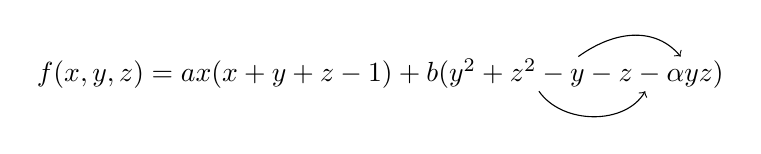
\begin{tikzpicture}
\node[anchor=west] at (0,0) {$f(x,y,z)=ax(x+y+z-1)+b(y^2+z^2-y-z-\alpha yz)$};
\draw[->] (7.0,.22) .. controls (7.5,.58) and (8.0,.58) .. (8.3,.22);
\draw[->] (6.5,-.22) .. controls (6.8,-.65) and (7.6,-.65) .. (7.85,-.22);
\end{tikzpicture}}
% source lines 13-16
\[
\begin{aligned}
f(\unsure{a|\underline a|\widehat a}s_2)=0\quad\text{i.e.}\quad
&a\alpha'(-\alpha')+b\Bigl(\underbrace{\deleted{\unsure{\alpha^{\prime 2}+\alpha'}}\inserted{\unsure{\alpha'(\alpha'+1)|\alpha'(\alpha+1)}}}_{1}+(1-\alpha')(-\alpha')\\
&\hspace{6em}-\underbrace{\alpha(-\alpha')}_{1}(1-\alpha')\Bigr]=0\\
&\underbrace{\hphantom{\alpha^{\prime 2}+\alpha'+(1-\alpha')(-\alpha')-\alpha(-\alpha')(1-\alpha')}}_{\deleted{\alpha'}-\deleted{\alpha'}+\alpha^{\prime 2}}\quad\deleted{\unsure{=0}}\\
&-(\alpha^{\prime 2})a+\alpha^{\prime 2}b=0\qquad\boxed{b=a}
\end{aligned}
\]
% source line 17
\[
f(x,y,z)=aq(x,y,z)
\]
% source lines 18-19
Il reste à vérifier $q(as_0)=q(as_1)=q(as_2)=\unsure{0}$.

Mais c'est OK car $q$ \unsure{invariante}\ldots


\scanpage{103}
% archive sheet number: 102
% source line 01
La partie homogène de $q$ est
% source line 02
\[
q_0(x,y,z)=x^2+y^2+z^2-\alpha yz+zx+xy\tag*{(19)}
\]
% source line 03
dont la matrice est
% source lines 04-06
\[
\deleted{\unsure{\widetilde q_0|\overrightarrow{q_0}}}
\begin{pmatrix}2&1&1\\1&2&-\alpha\\1&-\alpha&2\end{pmatrix}\tag*{(20)}
\]
% source lines 07-08
de discriminant
\[
\begin{aligned}
\delta&=\underline{8}-2\alpha-\underline{2}-2\alpha^2-\underline{2}\\
&=4-2(\underbrace{\alpha^2+\alpha}_{1})=2
\end{aligned}
\]
% source line 09
\[
\delta=2\qquad\text{donc}\qquad\underline{\delta'=1}\tag*{(21)}
\]
% source line 10
Forme quadratique donc \uuline{partout}, \uline{inversible}!

% source lines 11-12
Quant au discriminant de $q$ homogénéisé par une variable $t$
% source line 13
\[
q(x,y,z,t)=x^2+y^2+z^2-\alpha yz+zx+xy-t(x+y+z)
\]
% source line 14
c'est le déterminant de la matrice
% source lines 15-18
\[
\unsure{\widetilde q|\overrightarrow q}
\begin{pmatrix}
2&1&1&-1\\
1&2&-\alpha&-1\\
-\alpha&-1&2&-1\\
-1&-1&-1&0
\end{pmatrix}\tag*{(22)}
\]
% source lines 19-22; darker correction and additions at the foot
dont le discriminant \deleted{(sauf erreur de calcul)} est
$\deleted{\boxed{\alpha'}}\inserted{-\alpha-3}$,
\deleted{donc aussi \unsure{inv.} partout. Donc l'icosaèdre est inscrit}
\inserted{$\unsure{N|\mathcal N}(-\alpha-3)=5$ i.e. sauf en car. $5$ (\uline{NB} en car. $5$, l'icosaèdre est \unsure{inscrit} dans une sphère de rayon nul, donc quadrique \uline{sing.}!)}


\scanpage{104}
% archive sheet number: 103
% Source scan is upside down; transcription follows the writing after a 180-degree rotation.
% Three long oblique cancellation strokes cross the page.
% source rotated lines 01-02
\[
\deleted{W_T^+\simeq\mu_{nT}}\qquad\deleted{V_T\simeq D\oplus D^{-1}}
\]
\deleted{$\deleted{\unsure{\zeta|\xi}}\ \zeta\in\Gamma(\mu_{nT})$ opère sur $V_T$ par $\zeta\mathbin{.}(x,y)=(\zeta x,\zeta^{-1}y)$}
% source rotated upper left diagram
\diagram{\begin{tikzcd}[ampersand replacement=\&]
\deleted{T}\arrow[r,dash]\arrow[d]\&\deleted{T\times_S\Omega}\arrow[d,dash]\\
\deleted{S}\&\deleted{\Omega}\arrow[l,"{\deleted{\deleted{\unsure{\sigma}}}}"']
\end{tikzcd}}
% source rotated lines 03-06, central and right formulas
\[
\begin{aligned}
\deleted{\mu^*_{n\,T\times_S\Omega}\ni\zeta}&\qquad\deleted{\sigma_T\sigma_\omega}\\
&\deleted{\sigma_T\zeta=\zeta^{-1}\qquad\sigma_\omega\zeta=\zeta^{-1}}\\
&\deleted{\sigma_T\sigma_\omega\zeta=\zeta}\\
\deleted{\mu^*_{n\,\unsure{T\wedge\Omega|T\times\Omega}}}&
\end{aligned}
\]
% source rotated lines 07-10
\deleted{1) Module quadratique de rang $2$ non dég $(V,q)$}

\deleted{2) Section de ${\unsure{\Sigma|Z}}^{(q)}/\mu_n^{(q)}$}

\deleted{3) rev. étale quadratique $\Omega$ de $S$ et iso $\mu_{n\Omega}^{(q)}\simeq(\unsure{\mathbb Z/n\mathbb Z|\mathbb Z/2\mathbb Z})_\Omega$}

\deleted{\deleted{\unsure{4}}}
\deleted{(i.e. section de $\mu_{n\Omega}^{(q)*}$}

% source rotated middle left: repeatedly cancelled diagram sketch
\diagram{\unsure{\begin{tikzcd}[ampersand replacement=\&,row sep=small,column sep=small]
\deleted{\deleted{\unsure{T}}}\arrow[d,dash]\arrow[dr,dash]\&\deleted{\unsure{T|F}}\arrow[dl]\arrow[dr,bend left]\\
\deleted{S}\arrow[rr,bend right]\&\&\deleted{\Omega}\arrow[ll,bend right]\arrow[ul,bend left]
\end{tikzcd}}}
% source rotated middle centre
\diagram{\begin{tikzcd}[ampersand replacement=\&,row sep=small]
\deleted{T}\arrow[d,dash]\&\deleted{,}\&\deleted{\unsure{\mathscr A|\mathcal A}}\arrow[d,dash]\&\deleted{1}\\
\deleted{S}\&\&\deleted{\unsure{\mathscr O_S|\mathcal O_S}}\&
\end{tikzcd}}
% source rotated middle right
\[
\begin{aligned}
&\deleted{\zeta+\zeta^{-1}=c}\\
&\deleted{\zeta^2-c\zeta+1=0}\\
&\deleted{\zeta=\frac{c\pm\sqrt{c^2\unsure{-|+}4}}{}}\qquad
\deleted{\begin{gathered}c^2=4\\c=\pm2\end{gathered}}\\
&\hspace{13em}\deleted{\zeta=\zeta^{-1}}\\
&\hspace{13em}\deleted{\zeta^{\unsure{n|2}}\ne1}
\end{aligned}
\]
% source rotated middle left, unfinished second diagram
\diagram{\begin{tikzcd}[ampersand replacement=\&,row sep=small,column sep=small]
\deleted{T}\arrow[d,dash]\&{}\\
\deleted{S}\arrow[ur,dash]\&{}
\end{tikzcd}}
% source rotated lines 11-16
\deleted{\deleted{4) $c$ \unsure{sat.}}}

\deleted{1) $c\in\Gamma(S,\mathscr O_S)$ satisfaisant $\Phi_n(c)=0$}

\deleted{[$\Rightarrow$ rev. quadratique $R$ de $S$}
\[
\deleted{[\operatorname{Spec}\mathscr O_S[X]/(X^2-cX+1)])}
\]
\deleted{avec \deleted{\unsure{unique}} $\zeta\in\Gamma(R,\mu^*_{nR})$}
\[
\deleted{\sigma_R\zeta=\zeta^{-1}\qquad]}
\]
\deleted{\deleted{2) Rev}}
% source rotated bottom left
\[
\deleted{\mathscr O_S^2\quad\mu_n\ \text{opère par}\quad\lambda x,\lambda^{-1}x}
\]
\[
\deleted{\mu_n\mathbin{.}(1,1)}
\]
\(\deleted{\bigg)}\)
% source rotated bottom right, scheme and algebra columns
\diagram{\begin{tikzcd}[ampersand replacement=\&,row sep=small]
\deleted{R}\arrow[d,dash]\&\deleted{\mathscr A=\mathscr O_S[X]/(X^2-cX+1)}\arrow[d,dash]\\
\deleted{S}\&\deleted{\mathscr O_S}
\end{tikzcd}}


\scanpage{105}
% archive sheet number: 104
% printed form: blank music staves, running vertically in the scan
% source lines 01-04
\[
\begin{aligned}
\Delta_1&=\det\begin{pmatrix}1&1&-1\\2&-\alpha&-1\\-\alpha&2&-1\end{pmatrix}
=\alpha+\alpha-\deleted{4}-(-\alpha^2)\\
&\hspace{18em}-\deleted{(-2)}-\deleted{(-2)}\\
&=2\alpha+\alpha^2=\alpha+1=-\alpha'
\end{aligned}
\]
% source lines 05-08
\[
\begin{aligned}
\Delta_2&=\det\begin{pmatrix}2&1&-1\\1&-\alpha&-1\\1&2&-1\end{pmatrix}
=\underset{\cdot}{2\alpha}-\underset{\cdot}{2}-\deleted{1}-\underset{\cdot}{\alpha}-\deleted{(-1)}\\
&\hspace{18em}-\underset{\cdot}{(-4)}\\
&=\alpha+2
\end{aligned}
\]
% source lines 09-12
\[
\begin{aligned}
\text{\uuline{\uline{$\Delta_3$}}}&=\det\begin{pmatrix}2&1&-1\\1&\unsure{2}&-1\\1&-\alpha&-1\end{pmatrix}
=-\underset{\cdot}{4}+\underset{\cdot}{\alpha}-\deleted{1}-\underset{\cdot}{(-2)}\\
&\hspace{18em}-\underset{\cdot}{2\alpha}-\deleted{(-1)}\\
&=-2-\alpha
\end{aligned}
\]
% source lines 13-15; abandoned determinant prefix and curved redirecting arrow
\diagram{\begin{tikzcd}[ampersand replacement=\&,column sep=small,row sep=small]
\deleted{\det(\quad)=}\arrow[r,bend left]\&{}\\
\Delta_1-\Delta_2+\Delta_3\&{}\arrow[ul,phantom]
\end{tikzcd}}
\[
\begin{aligned}
&=\underbrace{-\alpha'-\alpha}_{1}-2-\alpha\\
&=-1-\alpha=\alpha'
\end{aligned}
\]
% source left margin, two lines written sideways and crossed through
% margin note written sideways
\margin{\deleted{\unsure{dérivée|dessin} sur $X_{\unsure{i|0}}$, \unsure{car|en} \unsure{ici|id.} \illegible{3} \unsure{les} \illegible{1} \unsure{un} \illegible{1}}}


\scanpage{106}
% archive sheet number: 105
% Page read after a quarter-turn; only the indicated passages are cancelled.
% source 01, top
Mod. loc. libre de rang $2$, ---.
% source 02, top, replacement above the cancelled identification
\[
\unsure{\mathfrak g|\mathscr G}\simeq
\deleted{\unsure{\operatorname{End}(F)|\operatorname{Ad}(F)}\unsure{\simeq|\otimes}
\check F\otimes F=\operatorname{End}_{\unsure{\mathscr O_S|\mathcal O_S}}(F)}
\inserted{\operatorname{Sym}^2(F)\otimes(\det F)^{-1}
\simeq\operatorname{Sym}^2\check F\otimes\det F}.
\]
% source 03, top right
\[
\deleted{\check F\simeq\unsure{F|\check F}\otimes(\det F)^{\unsure{-1|1}}}
\]
% source 04, top, cancelled continuation
\deleted{(\unsure{Morphismes|éléments} \unsure{sans} de trace nulle) avec le crochet habituel}
\[
\deleted{[X,Y]=XY-YX.}
\]
% source 05, upper left, added beside the cancelled block
\[
X\subset\operatorname P[\mathfrak g]=\operatorname P(\check\Omega).
\]
% source 06, upper left
\[
\begin{aligned}
\Omega&=\check{\mathfrak g}\\
&=\Gamma^2(\check F)\otimes(\det F)^{\unsure{2|1}}\\
&=\operatorname{Bil}\operatorname{sym}(F,F;\det F^{\unsure{2|1}}).
\end{aligned}
\]
% source 07, upper middle, crossed block
\deleted{La fonction dét sur \uline{$\operatorname{End}(F)$} est quadratique, sa restriction à $\mathfrak g$ est une}
% source 08, middle, live replacement below the cancelled block
On a une \inserted{forme quadratique} canonique (le discriminant)
\inserted{(au \unsure{facteur} \unsure{4|2|1})}
% source 09, middle
\diagram{\begin{tikzcd}[ampersand replacement=\&]
\deleted{\operatorname{Sym}^2(F)}\inserted{\Omega}
\arrow[r,"\delta"]\&
\deleted{(\det F)^{\otimes2}}\inserted{\mathscr O_S}
\end{tikzcd}}
% source 10, middle
donc
\diagram{\begin{tikzcd}[ampersand replacement=\&]
\mathfrak g=\operatorname{Sym}^2(F)(\det F)^{-1}
\arrow[r,"Q"]\&\mathscr O_S
\end{tikzcd}}
% source 11, middle, words above a long linking brace
(\unsure{On a aussi|On aura aussi|Et on aura}, la forme de \unsure{Casimir}
\inserted{\unsure{est déf.}, à c\textsuperscript{te} près, l'inverse de}
\unsure{$\cdots$|$Q$|$\delta$}). Si \unsure{on a}
% source 12, lower middle
une base de $F$, $F\simeq\mathscr O_S^2$, d'où base de $\det F$,
$\operatorname{Sym}^2F$ \unsure{---}, alors $\mathfrak g$ s'identifie au Module
\inserted{\unsure{bil. sym.}}
des formes
\[
\unsure{-a|a}xx'+b(xy'+x'y)+cyy',
\]
% source 13, bottom
et $\delta$ \unsure{est} la forme
\[
\deleted{b^2-ac}\inserted{\unsure{q\longmapsto ac-b^2|q\longmapsto b^2-ac}}.
\]
% source 14, bottom, cancelled prose and continuation
\deleted{\unsure{Si} $2$ est \unsure{inv.} (et de \illegible{1}
\unsure{canon.} \unsure{complétée} la trivialisation de
$\det\Omega\simeq\det\Gamma^2\check F\,(\det F)^3$
(\unsure{en bas}) est \unsure{bien définie}}
\[
\deleted{\simeq\unsure{\mathscr O_S|\otimes}\,(\det F)^{-3}\det F^3\simeq\mathscr O_S.}
\]
% source 15, left margin, alongside the lower half
% margin note written sideways
\margin{et vérifier que la \unsure{conique|courbe}
\unsure{est définie} par le discriminant \unsure{réduit} $\delta'(Q)$ ---}


\scanpage{107}
% archive sheet number: 106
% source 01, top; the rest of the sheet is blank
\deleted{\unsure{dans|donc} une} \uline{quadrique lisse} en \unsure{tt|tte} dimension !


\scanpage{108}
% archive sheet number: 107
% source 01-04, top
\uline{NB} Est-il clair que la condition $\alpha^2+\alpha-1=0$
est \uline{\unsure{suffisante|suffisant}} pour avoir une représentation
de l'icosaèdre ? On aura une représentation affine du gr.
% source 05-06, top
\[
\Gamma'=\left\{\sigma_0,\sigma_1,\sigma_2\ \left|\
\begin{aligned}
\sigma_0^2=\sigma_1^2=\sigma_2^2&=(\sigma_0\sigma_1)^3=(\sigma_1\sigma_2)^{\unsure{6|5}}\\
&=(\sigma_0\sigma_2)^2=1
\end{aligned}\right.\right\}.
\]
% source 07-09, upper middle
\unsure{Ce|Rque} groupe \deleted{\unsure{présenté}} admet $\Gamma$ comme
groupe quotient. Si on \deleted{\unsure{savait}}\inserted{utilise}
$\Gamma'\simeq\Gamma$ \unsure{---} \unsure{qu'on} connaît.
% source 10-13, middle
Sinon il faut une vérification un peu emmerdante
(mais de pure routine) que \deleted{\unsure{les}}\inserted{l'ens.}
des six points $s_0,s_1,s_2,s_3$, $s'_3,s''_3$ et leurs
``antipodiques'' \unsure{définis|definis} ``a priori'' \unsure{sont|est} stable sous
$\sigma_0,\sigma_1,\sigma_2$ (i.e. sous $\Gamma'$) et
\deleted{\unsure{que}} plus précisément que les op. des
$\sigma_0,\sigma_1,\sigma_2$ sur l'ens. de ces $12$ pts ``est'' la
``$=$'' que l'op. sur les $12$ pts de l'icos. comb. $\unsure{\Pi|T}$ ....
% source 14, separator
\figure{\begin{tikzpicture}\draw (0,0)--(2,0);\end{tikzpicture}}
% source 15-16, bottom
Ici $\sigma_0,\sigma_1,\sigma_2$ sont des réflexions. Les
hyperplans correspondants sont \deleted{\unsure{en}}
% source 17-19, bottom
\[
\left\{\begin{aligned}
H_0&:\quad 2x+y+z-1=0\\
H_1&:\quad -x+y+\alpha'z=0\\
H_2&:\quad \deleted{\unsure{\alpha|a}}y-z=0
\end{aligned}\right.
\]


\scanpage{109}
% archive sheet number: 108
% source 01-05, top
comme coordonnées affines et \deleted{\unsure{les}} exprimons
$\sigma_0,\sigma_1,\sigma_2$ p.r. à ces coordonnées --- pour
$\sigma_0,\sigma_2$ les coefficients sont des entiers bien déterminés
(les \unsure{signes|lignes} : $0$ ou $\pm1$) pour $\sigma_1$ il y a
des ``modules'' indéterminés $\lambda,\mu,\unsure{\nu|\gamma}$ satisfaisant
% source 06, upper middle
\[
\left\{\begin{aligned}
\nu^2&=1\\
\mu&=-\nu\lambda
\end{aligned}\right.\qquad\text{exprimant }\sigma_1^2=1
\]
% source 07, upper middle
puis $\nu=1$ (exprimant $u^3=\operatorname{id}$)
% source 08, upper right, corrected explanation
et enfin $\lambda^2+\lambda-1=0$
\deleted{(\unsure{car} $v=\sigma_1\sigma_2$, $v^{\unsure{5|6}}=\operatorname{id}$)}
\inserted{exprimant que $v^{\unsure{5|6}}=\operatorname{id}$.}
% source 09, middle, cancelled line
\deleted{On a fait \unsure{les calculs|le calcul} dans le cas $\nu=1$}
% source 10, middle, cancelled start
\deleted{$\mu=-\lambda$ (\unsure{qui est} \unsure{rappelé})}
% source 11-15, middle
--- au lieu de $\lambda$ on écrit aussi $\alpha'$ ... et on a trouvé,
exprimant $(\sigma_1\sigma_2)^5=\operatorname{id}$, l'équation
(en $\alpha$, ou $\alpha'$, au choix)
\[
\alpha^2+\alpha-1=0
\]
en termes de laquelle on a vérifié la fidélité.
% source 16-19, lower half, entire passage cancelled by large crosses
\deleted{Pour bien faire, il faudrait aussi traiter le cas où on ne suppose
pas $\nu=1$ i.e. \unsure{on n'impose pas|on ne supposerait pas}
$\sigma_1$ une réflexion (\unsure{en} car. rés. $\ne2$,
\unsure{cel.} revient à prendre $\nu=\deleted{\unsure{1|+1}}-1$)}
% source 20-22, cancelled continuation with local changes
\deleted{Considérons le \deleted{point} plan de $s_1,s_2,s_3$, soit $P$,
\inserted{d'équation $x+y+z=0$}
\deleted{\unsure{puisqu'}}\inserted{\unsure{notons qu'}} il contient
$s'_3=(\lambda,\mu,\nu)$ i.e. \deleted{\unsure{que} $\lambda+\mu+\nu=0$}
on a}
% source 23-26, bottom, all displays cancelled
\[
\deleted{\lambda+\mu+\nu=1}
\]
\deleted{i.e.}
\[
\deleted{\lambda-\nu\lambda+\nu=1\qquad\text{i.e. }\deleted{(\lambda-\nu\lambda)+\nu}}
\]
\[
\deleted{(\quad)\qquad(\lambda-1)(1-\nu)=0\qquad?}
\]
% source 27, bottom, locally crossed as well
\deleted{\deleted{Mais en fait, si $\nu\ne1$}}


\scanpage{110}
% archive sheet number: 109
% source 01-04, top
Si une réalisation est acceptable, \deleted{\unsure{les}} \unsure{prenons|prenant}
quatre pts distincts $s_0,s_1,s_2,s_3$ dont les trois premiers sont sur
une $=$ face, leurs réal. géom. sont aff\textsuperscript{t}
\unsure{indépendantes|indépendants}.
% source 05-08, upper middle, revised definition
\deleted{Considérons} Une représentation \inserted{est dite}
\deleted{\uuline{acceptable}} \deleted{\unsure{dans le}}
\inserted{\uline{régulière}} si \inserted{elle est acceptable et si}
pour \unsure{tt|tout} $g\in\Gamma$ $\exists!\,g_E$ qui est un affine de $E$
qui \unsure{le|la} prolonge.
% source 09-11, middle
\deleted{\unsure{Pour en faire}}\inserted{C'est une}
\deleted{\unsure{on définit} les repr. acceptables}
propriété de l'application $\unsure{\rho_S|\rho_s}$ en fait, et
n'implique pas $\rho_S(S)$ engendre affinement $E$.
% source 12, left slanted margin linked to the definition
% slanted
\margin{$\times$ \uline{NB} la condition ``acceptable'' revient à exiger que
$\rho_S$ \unsure{soit} un \unsure{point|plgt}
$\unsure{\operatorname{Conv}S|\operatorname{Conf}S}\to E$, ou encore que
$\rho_S(S)$ ne soit pas contenu dans une droite...}
% source 13, middle
\uline{Prop.} Une représentation régulière est \uline{fidèle}.
% source 14-16, lower middle
Soit $\deleted{(\unsure{\delta_0|\sigma_0},\delta_1,\delta_2)}$
$(\sigma_0,\sigma_1,\sigma_2)\in\Gamma$ les symétries fond. associées
au repère, $\deleted{\unsure{\varphi|s}}s_0$ le sommet origine,
% source 17, lower middle
\[
s_1=\sigma_0s_0,\quad s_2=\sigma_1s_1,\quad s_3=\sigma_2s_2
\]
% source 18-20, lower middle
\deleted{Je dis que}
Je dis que $s_0,s_1,s_2,s_3$ sont aff\textsuperscript{t} indép. :
On sait déjà par hyp. que $s_0,s_1,s_2$ le sont.
% source 21-24, bottom
Si on avait $s_3\in P:=\operatorname{Pl}(s_0,s_1,s_2)$, il est visible que
$P$ --- qui est déjà invariant par $\sigma_0,\sigma_1$ --- serait invariant
par $\sigma_2$ $\deleted{(\unsure{\sigma_2|\sigma_1})}$ puisque
\[
\sigma_2(P)=\operatorname{Pl}(\sigma_2(s_0)=s_0,\ \sigma_2(s_1)=s_1,\
\sigma_2(s_2)=s_3)=P
\]
% source 25, bottom, continuation stops at the end of this scan
Ceci étant, on peut \deleted{\unsure{faire}} choisir $s_0,s_1,s_2,s_3$
